\documentclass[11pt]{article}

% ---------------------------------------------------------------------------
%  Parallelising timed-automata reachability: OpenMP and Metal GPU backends
% ---------------------------------------------------------------------------
\usepackage[utf8]{inputenc}
\usepackage[T1]{fontenc}
\usepackage{lmodern}
\usepackage[a4paper,margin=2.4cm]{geometry}
\usepackage{amsmath,amssymb,amsthm}
\usepackage{booktabs}
\usepackage{xcolor}
\usepackage{graphicx}
\usepackage{caption}
\usepackage{subcaption}
\usepackage{algorithm}
\usepackage{algpseudocode}
\usepackage{listings}
\usepackage{microtype}
\usepackage{tikz}
\usepackage{pgfplots}
\pgfplotsset{compat=1.18}
\usetikzlibrary{arrows.meta,positioning,calc,fit,backgrounds,shapes.geometric,
                decorations.pathreplacing,shadows.blur,matrix}
\usepackage[hidelinks]{hyperref}
\usepackage[nameinlink]{cleveref}

% ---- palette --------------------------------------------------------------
\definecolor{cpu}{HTML}{2C6E9B}     % blue   -- host / CPU
\definecolor{gpu}{HTML}{B5651D}     % orange -- GPU
\definecolor{acc}{HTML}{3F7A3F}     % green  -- accents
\definecolor{soft}{HTML}{F1F4F8}
\definecolor{softg}{HTML}{FBEFE3}
\definecolor{codebg}{HTML}{F7F7F4}

% ---- tikz styles ----------------------------------------------------------
\tikzset{
  box/.style   ={rounded corners=2pt, draw=black!55, thick, align=center,
                 font=\small, inner sep=5pt, minimum height=8mm},
  cpubox/.style={box, fill=soft,  draw=cpu!70},
  gpubox/.style={box, fill=softg, draw=gpu!75},
  lane/.style  ={rounded corners=3pt, draw=black!25, thick, inner sep=7pt},
  flow/.style  ={-{Stealth[length=2.4mm]}, thick, draw=black!65},
  dflow/.style ={-{Stealth[length=2.4mm]}, thick, draw=black!45, dashed},
  lbl/.style   ={font=\scriptsize\itshape, text=black!60},
}

% ---- listings -------------------------------------------------------------
\lstset{
  basicstyle=\ttfamily\footnotesize, backgroundcolor=\color{codebg},
  breaklines=true, columns=fullflexible, keepspaces=true, frame=single,
  rulecolor=\color{black!20}, framesep=4pt, xleftmargin=4pt,
  commentstyle=\color{acc}, keywordstyle=\color{cpu}\bfseries,
  language=C++, showstringspaces=false, morekeywords={kernel,device,__global__,constant,thread}
}

\newtheorem{proposition}{Proposition}
\newcommand{\dk}{\ensuremath{\mathit{dk}}}
\newcommand{\aluleq}{\ensuremath{\preceq_{\mathrm{aLU}}}}
\newcommand{\code}[1]{\texttt{\small #1}}

\title{\bfseries Parallelising Timed-Automata Reachability:\\[2pt]
  \large A Shared-Memory (OpenMP) and a GPU (Metal/CUDA) Backend for a Timed-CTL Model Checker}
\author{PTCTLMC Project}
\date{\today}


% ---- extra packages used by this paper ------------------------------------
\usepackage{multirow}
\usetikzlibrary{patterns}

% ---- aliases: keep local figure code readable while using the house palette -
\colorlet{cA}{cpu}
\colorlet{cB}{gpu}
\colorlet{cC}{acc}
\colorlet{cD}{cpu!60!black}
\definecolor{cGrey}{HTML}{7F8C8D}

% ---- macros ---------------------------------------------------------------
\providecommand{\Zone}{\mathcal{Z}}
\providecommand{\DBM}[1]{\mathbf{D}_{#1}}
\providecommand{\Passed}{\mathit{Passed}}
\providecommand{\dk}{\mathit{dk}}
\providecommand{\aLU}{\ensuremath{\preceq_{\mathit{LU}}}}
\providecommand{\tool}{\textsc{Ptctlmc}}
\providecommand{\uppaal}{\textsc{Uppaal}}
\providecommand{\ltsmin}{\textsc{LTSmin}}
\providecommand{\opaal}{\textsc{opaal}}


\title{Why GPUs Lose at Zone-Graph Exploration: Ten Measured Attempts on Apple Silicon}
\author{}
\date{}

\begin{document}
\maketitle

\begin{abstract}
Symbolic reachability for timed automata generates millions of independent successor
computations, which makes it look like an ideal GPU workload. We report that it is not, and
--- more usefully --- we identify the mechanism. We implemented GPU successor generation and
per-state zone merging in Metal, in \emph{three} different DBM representations and across ten
measured configurations, and compared each against an optimised 12-core CPU implementation of
the same algorithm. Every GPU component is slower than its CPU counterpart: expansion
$1400$\,ms versus $491$\,ms, merging $258$--$571$\,ms versus $100$\,ms; an adaptive router
given a free per-level choice selects the CPU on $122$ of $124$ levels. We refute the two
hypotheses a practitioner would reach for first. Branch divergence is \emph{not} the cause:
$100.0\%$ of lanes survive to do full work on Viking and $71.5\%$ on Fischer, so stream
compaction would recover nothing. Instead the cause is a \emph{working-set dilemma}: a DBM is
too large to hold in registers and too large to hold on-chip at useful occupancy. We further
show that no change of representation escapes this, because one-zone-per-thread already
extracts all available parallelism, and any cooperative mapping must beat a $32\times$
deficit with at most $\mathit{dim}\times$ intra-zone parallelism. We close by scoping the
result: the dominant cause is a threadgroup-memory capacity limit that datacenter GPUs relax
by $7\times$, so the honest claim is about unified-memory Apple GPUs, not about GPUs in
general.
\end{abstract}

\section{Introduction}
\label{sec:intro}

Zone-graph reachability appears tailor-made for a GPU. A BFS level contains millions of
$(\text{state},\text{edge})$ pairs; each is expanded independently; the arithmetic is small
dense integer matrix work. Yet across a sustained implementation effort we were unable to
make a GPU implementation beat a 12-core CPU implementation of the same algorithm on the same
chip, and the reasons turned out to be interesting enough to report.

This paper is a negative result with a mechanism. Its value is threefold. First, it refutes,
\emph{on measurement rather than intuition}, the hypothesis most practitioners (including the
authors) reach for first --- branch divergence --- and thereby saves the reader from
implementing the standard fix. Second, it identifies the actual cause and shows it is not a
coding failure but a consequence of the algorithm's shape. Third, it delimits the claim
precisely: the dominant cause is a hardware capacity that a datacenter GPU relaxes, so the
result should not be read as ``GPUs cannot do this''.

\paragraph{Contributions.}
\begin{itemize}
\item Three GPU DBM representations, all implemented and validated against exact
\uppaal{} state counts (Sect.~\ref{sec:reps}).
\item An adaptive per-level CPU/GPU merge router, whose selections are themselves a
measurement instrument (Sect.~\ref{sec:adaptive}).
\item A refutation of the divergence hypothesis and identification of the working-set
dilemma (Sect.~\ref{sec:why}), plus a counting argument showing no representation escapes it
(Sect.~\ref{sec:cooperation}).
\item A scoped outlook for datacenter GPUs (Sect.~\ref{sec:h100}).
\end{itemize}

\section{Background and GPU Design}
\label{sec:design}

A symbolic state pairs a discrete location vector with a zone stored as a
$(m{+}1)\times(m{+}1)$ Difference Bound Matrix in canonical form. The successor pipeline for
one $(\text{state},\text{edge})$ pair is shown in Fig.~\ref{fig:kernel}: integer guard, clock
guard, resets, combined invariant, delay, invariant again, inactive-clock reset,
extrapolation, emptiness. Integer guards are evaluated \emph{host-side} while the work list
is built, so the kernel receives only pairs whose discrete part is already known feasible ---
a fact that matters in Sect.~\ref{sec:why}.

\begin{figure}[t]
\centering
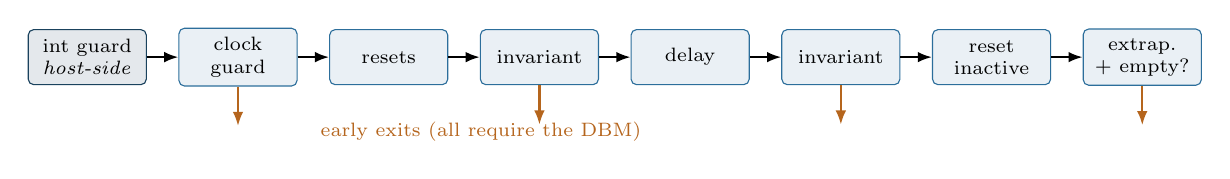
\begin{tikzpicture}[font=\small,
  st/.style={draw, rounded corners=2pt, minimum height=7mm, minimum width=15mm, align=center,
             font=\scriptsize, fill=cA!10, draw=cA},
  host/.style={st, fill=cD!12, draw=cD},
  ar/.style={-{Latex[length=1.8mm]}, thick},
  ex/.style={-{Latex[length=1.8mm]}, cB, thick}]

\node[host] (ig) at (0,0) {int guard\\\textit{host-side}};
\node[st, right=4mm of ig] (cg) {clock\\guard};
\node[st, right=4mm of cg] (rs) {resets};
\node[st, right=4mm of rs] (iv) {invariant};
\node[st, right=4mm of iv] (dl) {delay};
\node[st, right=4mm of dl] (iv2) {invariant};
\node[st, right=4mm of iv2] (ri) {reset\\inactive};
\node[st, right=4mm of ri] (ex) {extrap.\\+ empty?};

\foreach \a/\b in {ig/cg, cg/rs, rs/iv, iv/dl, dl/iv2, iv2/ri, ri/ex} \draw[ar] (\a) -- (\b);
\foreach \n in {cg, iv, iv2, ex} \draw[ex] (\n.south) -- ++(0,-5mm);
\node[font=\scriptsize, cB] at (5.0,-0.95) {early exits (all require the DBM)};
\end{tikzpicture}
\caption{Per-work-item successor pipeline. Only the first stage is DBM-free, and it already
runs on the host, so a cheap GPU pre-filter has nothing left to reject.}
\label{fig:kernel}
\end{figure}

\subsection{Three DBM representations}
\label{sec:reps}

We implemented three mappings of a zone onto the GPU (Fig.~\ref{fig:reps}), all producing
identical, \uppaal{}-exact state counts.

\begin{description}
\item[R1: private dense matrix (baseline).] One work item per thread; the zone lives in a
per-thread array \texttt{int z[MAXDIM*MAXDIM]}. At $\mathit{MAXDIM}=24$ this is 2304\,B.
\item[R2: threadgroup-resident dense matrix.] One work item per thread, but the zone lives in
threadgroup (on-chip) memory, sized by the model's real $\mathit{dim}$ rather than
$\mathit{MAXDIM}$, with an odd stride to avoid bank conflicts.
\item[R3: row-distributed.] One work item per \emph{SIMD group}; lane $i$ owns row $i$ of the
matrix in registers. Per-lane footprint falls from $\mathit{dim}^2$ to $\mathit{dim}$ --- a
$24\times$ reduction. Floyd--Warshall obtains $d[k][\cdot]$ by \texttt{simd\_shuffle},
register-to-register; \emph{emptiness} folds through \texttt{simd\_any}.
\end{description}

\begin{figure}[t]
\centering
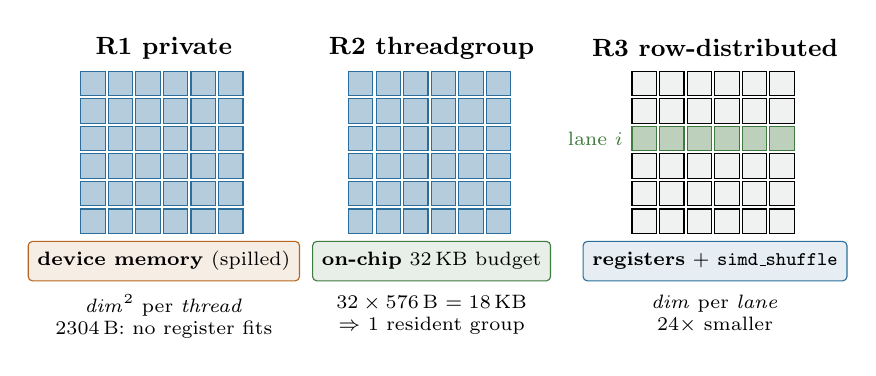
\begin{tikzpicture}[font=\scriptsize, node distance=3mm,
  cell/.style={draw, minimum size=3.1mm, inner sep=0pt, fill=cGrey!12},
  own/.style={cell, fill=cA!35, draw=cA},
  own2/.style={cell, fill=cC!35, draw=cC},
  lab/.style={font=\small\bfseries},
  mem/.style={draw, rounded corners=1.5pt, font=\scriptsize, minimum height=5mm}]

% R1
\node[lab] at (1.1,2.35) {R1 private};
\foreach \i in {0,...,5} \foreach \j in {0,...,5}
  \node[own] at (0.35*\j+0.2, 1.9-0.35*\i) {};
\node[mem, fill=cB!12, draw=cB, below=1mm of {(1.1,0.0)}, anchor=north] (m1)
  {\textbf{device memory} (spilled)};
\node[below=0.5mm of m1, align=center] {$\mathit{dim}^2$ per \emph{thread}\\2304\,B: no register fits};

% R2
\node[lab] at (4.5,2.35) {R2 threadgroup};
\foreach \i in {0,...,5} \foreach \j in {0,...,5}
  \node[own] at (0.35*\j+3.6, 1.9-0.35*\i) {};
\node[mem, fill=cC!12, draw=cC, below=1mm of {(4.5,0.0)}, anchor=north] (m2)
  {\textbf{on-chip} 32\,KB budget};
\node[below=0.5mm of m2, align=center] {$32\times576$\,B $=18$\,KB\\$\Rightarrow$ 1 resident group};

% R3
\node[lab] at (8.1,2.35) {R3 row-distributed};
\foreach \i in {0,...,5} \foreach \j in {0,...,5}
  \node[cell] at (0.35*\j+7.2, 1.9-0.35*\i) {};
\foreach \j in {0,...,5} \node[own2] at (0.35*\j+7.2, 1.9-0.35*2) {};
\node[left=1mm of {(7.15,1.9-0.7)}, cC, font=\scriptsize] {lane $i$};
\node[mem, fill=cA!12, draw=cA, below=1mm of {(8.1,0.0)}, anchor=north] (m3)
  {\textbf{registers} + \texttt{simd\_shuffle}};
\node[below=0.5mm of m3, align=center] {$\mathit{dim}$ per \emph{lane}\\$24\times$ smaller};
\end{tikzpicture}
\caption{Three DBM representations. R3 solves the footprint problem outright, and still loses
--- for the reason given in Sect.~\ref{sec:cooperation}.}
\label{fig:reps}
\end{figure}

\subsection{Adaptive CPU/GPU merge routing}
\label{sec:adaptive}

Per-discrete-state merging (\aLU{} subsumption plus convex union) is a second kernel: one
bucket per thread. Because bucket shape varies enormously between models, we route each BFS
level to whichever device is predicted faster. The router calibrates the throughput of each
path on early levels --- measuring $\mathit{work}/\mathit{ms}$ with
$\mathit{work} = \sum_b |b|^2$, the natural cost model for pairwise antichain folding ---
then routes each later level to the higher-throughput device, updating its estimate with an
exponential moving average (Fig.~\ref{fig:adaptive}).

The router is useful in its own right, but its scientific value here is as an
\emph{instrument}: given a free choice on every level, its selections are an unbiased
verdict on which device is actually faster.

\begin{figure}[t]
\centering
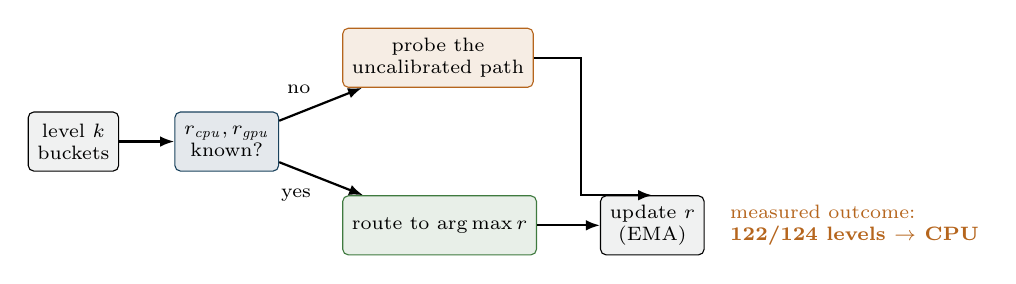
\begin{tikzpicture}[font=\small,
  b/.style={draw, rounded corners=2pt, minimum height=7.5mm, align=center, font=\scriptsize},
  ar/.style={-{Latex[length=1.8mm]}, thick}]
\node[b, fill=cGrey!12] (lvl) {level $k$\\buckets};
\node[b, right=7mm of lvl, fill=cD!12, draw=cD] (cal) {$r_{\mathit{cpu}},r_{\mathit{gpu}}$\\known?};
\node[b, above right=3mm and 8mm of cal, fill=cB!12, draw=cB] (probe) {probe the\\uncalibrated path};
\node[b, below right=3mm and 8mm of cal, fill=cC!12, draw=cC] (route) {route to
$\arg\max r$};
\node[b, right=8mm of route, fill=cGrey!12] (upd) {update $r$\\(EMA)};
\draw[ar] (lvl) -- (cal);
\draw[ar] (cal) -- node[above left, font=\scriptsize] {no} (probe);
\draw[ar] (cal) -- node[below left, font=\scriptsize] {yes} (route);
\draw[ar] (route) -- (upd);
\draw[ar] (probe.east) -- ++(6mm,0) |- (upd.north);
\node[right=2mm of upd, font=\scriptsize, align=left, cB]
  {measured outcome:\\\textbf{122/124 levels $\to$ CPU}};
\end{tikzpicture}
\caption{Adaptive per-level merge routing. Used as a measurement instrument, it selects the
GPU only for the single calibration probe on each model.}
\label{fig:adaptive}
\end{figure}

\section{Measurements}
\label{sec:meas}

All numbers are on an Apple M4 Pro: 8 performance + 4 efficiency CPU cores, a 16-core GPU
(${\approx}2000$ shader lanes), 24\,GB unified memory. Models are Viking N=15
($m{+}1=12$, so a $12\times12$ DBM $=576$\,B; $8\,355\,840$ successors) and Fischer N=10.

\begin{table}[t]
\centering
\caption{GPU components against their CPU counterparts. Every row favours the CPU.}
\label{tab:head}
\begin{tabular}{lrrl}
\toprule
Operation & GPU & CPU & Note \\
\midrule
Expansion (Viking 15) & 1400\,ms & \textbf{491\,ms} & CPU $2.85\times$ faster \\
Merge, zones written by GPU & 258\,ms & \textbf{100\,ms} & GPU's best case \\
Merge, zones written by CPU & 571\,ms & \textbf{100\,ms} & coherency penalty \\
Adaptive router's free choice & 2 levels & \textbf{122 levels} & of 124 total \\
\bottomrule
\end{tabular}
\end{table}

A consequence worth stating plainly: the configuration that is fastest on Fischer nominally
uses the Metal backend, but performs $100\%$ of its work on the CPU. Its advantage is
\emph{algorithmic} --- a bucketed, batched per-state merge over compact arrays --- and
removing the GPU from that configuration makes it faster still ($0.59$\,s $\to$ $0.42$\,s).
It must not be reported as GPU acceleration.

\section{Why: two refuted hypotheses and one real cause}
\label{sec:why}

\subsection{Divergence is not the cause}

The standard explanation is lockstep execution: lanes run in groups of 32, most edges fail
their guard early, and one survivor drags 31 idle lanes through the remaining pipeline. We
instrumented lane survival directly:

\begin{center}
\begin{tabular}{lrrr}
\toprule
Model & Work items & Survivors & Survive \\
\midrule
Viking N=15 & $8\,355\,840$ & $8\,355\,840$ & \textbf{100.0\%} \\
Fischer N=10 & $3\,317\,950$ & $2\,372\,190$ & 71.5\% \\
\bottomrule
\end{tabular}
\end{center}

On Viking there is \emph{no} early-exit divergence whatsoever. Stream compaction or wavefront
scheduling --- the standard remedy, and the idea we were about to implement --- would recover
$0\%$ there and at most $28\%$ on Fischer. Moreover the only DBM-free filter, the integer
guard, is already applied host-side (Fig.~\ref{fig:kernel}), so a cheap pre-pass has nothing
to reject. \emph{We report this specifically so that others do not implement it.}

\subsection{Arithmetic intensity is not (yet) the cause}

Each successor moves ${\approx}1152$\,B for ${\approx}2600$ integer operations:
$2.3$\,ops/byte against a roofline ridge point of ${\approx}10$, so the kernel is memory-bound
\emph{in character}. But the achieved rates are nowhere near that bound:

\begin{center}
\begin{tabular}{lrrr}
\toprule
& Rate & \% compute peak & \% bandwidth \\
\midrule
GPU expand (1400\,ms) & 5.97\,M succ/s & \textbf{0.5\%} & 2.5\% \\
CPU expand (491\,ms) & 17.0\,M succ/s & ${\approx}20\%$ (of CPU) & 7\% \\
\bottomrule
\end{tabular}
\end{center}

The bandwidth ceiling for this kernel is ${\approx}237$\,M succ/s, roughly $40\times$ above
what the GPU achieves. The GPU is limited by \emph{utilisation}, not by a physical roof: the
CPU runs at ${\approx}20\%$ of its peak while the GPU runs at $0.5\%$ of its own.

\subsection{The working-set dilemma}
\label{sec:dilemma}

Because Floyd--Warshall's $k$ loop is strictly sequential, there is almost no parallelism
\emph{inside} one zone, so every thread must own a whole zone. That creates a dilemma with no
good side, and we measured both horns (Table~\ref{tab:reps}).

\begin{table}[t]
\centering
\caption{Expansion time by representation. R3 cuts per-lane footprint $24\times$ and is the
slowest of the three.}
\label{tab:reps}
\begin{tabular}{llrr}
\toprule
& Representation & Viking N=15 & Fischer N=10 \\
\midrule
R1 & private dense (spills to device memory) & \textbf{1425\,ms} & \textbf{183\,ms} \\
R2 & threadgroup-resident dense & 1587\,ms & 277\,ms \\
R2$'$ & \quad + bank-conflict padding & 1575\,ms & 297\,ms \\
R3 & row-distributed across SIMD lanes & 2536\,ms & 351\,ms \\
\bottomrule
\end{tabular}
\end{table}

Keeping the zone \textbf{private} means 2304\,B per thread, far beyond the ${\approx}128$--$256$
registers a thread receives, so it spills to thread-local \emph{device} memory and all
${\approx}2600$ DBM operations per successor run at device-memory latency. Keeping it
\textbf{on-chip} costs $32 \times 576\,\text{B} = 18$\,KB of Apple's 32\,KB threadgroup
budget, leaving roughly one resident threadgroup per core: occupancy collapses and there is
nothing left with which to hide latency. R1 wins because sheer thread count buys more latency
hiding than on-chip residency buys in access speed.

\subsection{No representation escapes it}
\label{sec:cooperation}

R3 was designed to break the dilemma and does so on its own terms --- $\mathit{dim}$ ints per
lane, comfortably register-resident --- yet it is the slowest. The reason is a counting
argument, and it generalises to \emph{any} cooperative mapping.

One zone per \emph{thread} keeps $32$ independent zones in flight per SIMD group. Any scheme
that cooperates \emph{within} a zone --- R2's shared tile or R3's distributed rows --- processes
$1$ zone per SIMD group. Cooperation must therefore make a single zone more than $32\times$
faster merely to break even. The parallelism available inside one zone is only
$\mathit{dim}$-wide: at $\mathit{dim}=12$ that is 12 of 32 lanes busy, an immediate
$2.7\times$ loss, with a ceiling of $12\times$ before paying for \texttt{simd\_shuffle}
traffic and the serial $k$ loop. \textbf{Twelve-fold best case against a thirty-two-fold
deficit.} Both cooperative attempts lost, by different mechanisms, exactly as predicted.

This is the deepest reason a ``GPU-friendly representation'' does not exist here: the
workload's parallelism lives \emph{across} zones and is already fully exploited by the
simplest possible mapping. The dense matrix inherited from \uppaal{} is not what holds the
GPU back.

\subsection{Unified-memory coherency}

Finally, a hybrid in which the CPU expands and the GPU merges --- attractive because the two
phases favour different hardware --- is defeated by cache coherency. Identical merge work
costs 258\,ms when the zones were written by the GPU and 571\,ms when written by the CPU,
because the GPU must snoop them out of CPU caches. The moment the CPU produces the zones, the
GPU is the wrong consumer.

\section{Outlook: would a larger GPU change the answer?}
\label{sec:h100}

Partly, and the claim should be scoped accordingly. The dominant cause,
Sect.~\ref{sec:dilemma}, is a \emph{capacity} limit, and datacenter GPUs relax it
substantially (Table~\ref{tab:h100}). With 228\,KB of shared memory per SM one could hold
${\approx}390$ zones on-chip, so R2's failure mode largely disappears. Because the workload is
latency-bound with millions of \emph{independent} zones, absolute throughput should also
scale with GPU size even at unchanged utilisation; scaling crudely by lanes and bandwidth
suggests $50$--$70$\,M succ/s against our CPU's $17$\,M.

\begin{table}[t]
\centering
\caption{The dominant cause is substantially an Apple-Silicon capacity constraint.}
\label{tab:h100}
\begin{tabular}{lrr}
\toprule
& Apple M4 Pro & NVIDIA H100 \\
\midrule
Shared / threadgroup memory & 32\,KB per group & 228\,KB per SM \\
Memory bandwidth & 273\,GB/s (shared with CPU) & ${\approx}3.3$\,TB/s dedicated \\
Lanes & ${\approx}2\,000$ & ${\approx}16\,900$ \\
\bottomrule
\end{tabular}
\end{table}

What would \emph{not} improve: the serial $k$ loop, and the counting argument of
Sect.~\ref{sec:cooperation} (warps are also 32 lanes wide), so one-zone-per-thread remains the
right mapping --- merely a wider one. Coherency becomes \emph{worse} on a discrete GPU, since
PCIe transfers replace cache snooping unless the entire search is made GPU-resident, which in
turn requires a correct lock-free device-side hash table; our attempt at one produced
incorrect results because Metal Shading Language exposes only relaxed atomics, with no
acquire/release pairing for the publication step.

Two caveats for a fair follow-up: an H100 should be compared against a similarly priced CPU
(a 128-core server part, not 12 consumer cores), and GPU residency is a prerequisite rather
than an optimisation.

\section{Conclusion}
\label{sec:concl}

Across ten measured configurations and three DBM representations, GPU zone-graph exploration
on a unified-memory Apple GPU is slower than an optimised CPU implementation of the same
algorithm, component by component. The cause is neither branch divergence (refuted: $100\%$
lane survival) nor arithmetic intensity (refuted: $0.5\%$ of peak, $40\times$ from the roof),
but a working-set dilemma in which a DBM is simultaneously too large for registers and too
large for on-chip residency at useful occupancy --- and a counting argument that forecloses
the cooperative mappings that would otherwise escape it. We scope the result to
unified-memory GPUs with small threadgroup budgets, and identify the shared-memory capacity
of datacenter parts as the specific quantity that would have to change.


\begin{thebibliography}{8}
\bibitem{dalsgaard2012multicore}
Dalsgaard, A.E., Laarman, A., Larsen, K.G., Olesen, M.C., van de Pol, J.:
Multi-core reachability for timed automata. In: FORMATS. LNCS, vol. 7595, pp. 91--106.
Springer (2012)

\bibitem{behrmann2004tutorial}
Behrmann, G., David, A., Larsen, K.G.: A tutorial on Uppaal. In: SFM. LNCS, vol. 3185,
pp. 200--236. Springer (2004)

\bibitem{behrmann2006lower}
Behrmann, G., Bouyer, P., Larsen, K.G., Pel\'{a}nek, R.: Lower and upper bounds in zone-based
abstractions of timed automata. STTT \textbf{8}(3), 204--215 (2006)

\bibitem{laine2013megakernels}
Laine, S., Karras, T., Aila, T.: Megakernels considered harmful: Wavefront path tracing on
GPUs. In: High-Performance Graphics, pp. 137--143 (2013)

\bibitem{williams2009roofline}
Williams, S., Waterman, A., Patterson, D.: Roofline: An insightful visual performance model
for multicore architectures. Commun. ACM \textbf{52}(4), 65--76 (2009)
\end{thebibliography}

\end{document}
